\chapter{Work distribution}\label{ch:division_of_work}
This chapter describes the division of work on the application and the document.
The work distribution for the application is presented in \autoref{tab:division_of_work_on_the_application} and the work distribution for the document is presented in \autoref{tab:division_of_work_on_the_document}.
It is important to note that all parts of the project were worked on by both authors.
Each line in both the application source code and the document written by one of the authors was reviewed by the other author in a pull request.
Moreover, both authors made bug fixes and small changes to all parts of the project.
These tables only show who the main author of each part was.
Overall, the work was distributed evenly between the authors.
This can be seen in a screenshot from the GitHub repository in \autoref{fig:github_contributions}, which shows that the authors have the exact same number of commits.

\begin{figure}[h]
    \centering
    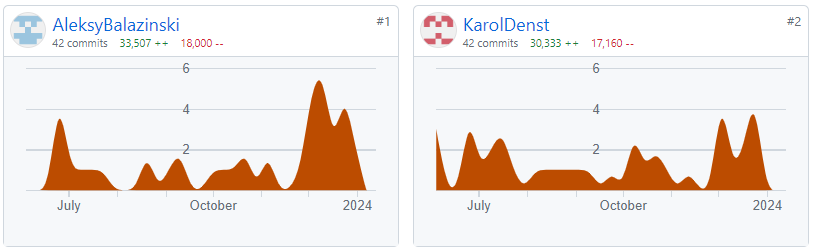
\includegraphics[width=0.8\textwidth]{chapters/work_distribution/resources/github_contributions.png}
    \caption{GitHub contributions}
    \label{fig:github_contributions}
\end{figure}

\begin{table}[h]
    \centering
    \begin{tabular}{|l|l|}
    \hline
    Task     & Author        \\ \hline
    Implementation of the game logic & Both \\
    Implementation of the graphics engine & Both \\
    Implementation of terrain editing & Both \\
    Implementation of the spherical geometry & Aleksy Bałaziński      \\
    Implementation of the hyperbolic geometry & Aleksy Bałaziński      \\
    Integration of the physics engine with the rest of the system & Aleksy Bałaziński      \\
    Implementation of the terrain generation & Karol Denst      \\
    Implementation of the user interface (HUD \& Menu) & Karol Denst      \\
    Implementation of character models and animations & Karol Denst      \\
    \hline
    \end{tabular}
    \caption{Work distribution for the application}
    \label{tab:division_of_work_on_the_application}
\end{table}
    
\begin{table}[h]
    \centering
    \begin{tabular}{|l|l|l|}
    \hline
    Chapter  & Section    & Author        \\ \hline
    \nameref{ch:introduction} &  & Both \\
    \nameref{ch:division_of_work} &  & Both \\
    \nameref{ch:functional_specification} & & Both \\
    \nameref{ch:theoretical_foundations} & \nameref{sec:non_euclidean_geometry} & Aleksy Bałaziński      \\
    \nameref{ch:theoretical_foundations} & \nameref{sec:theory_theory_marching_cubes} & Karol Denst      \\
    \nameref{ch:theoretical_foundations} & \nameref{sec:theory_theory_models} & Karol Denst      \\
    \nameref{ch:theoretical_foundations} & \nameref{sec:theory_theory_day_night_cycle} & Aleksy Bałaziński      \\
    \nameref{ch:theoretical_foundations} & \nameref{sec:theory_theory_lighting} & Aleksy Bałaziński      \\
    \nameref{ch:implementation} & \nameref{sec:technologies_selection} & Aleksy Bałaziński      \\
    \nameref{ch:implementation} & \nameref{sec:game_objects_management} & Aleksy Bałaziński      \\
    \nameref{ch:implementation} & \nameref{sec:implementation_terrain} & Karol Denst      \\
    \nameref{ch:implementation} & \nameref{sec:chunk-worker} & Aleksy Bałaziński      \\
    \nameref{ch:implementation} & \nameref{sec:implementation_rendering} & Aleksy Bałaziński      \\
    \nameref{ch:implementation} & \nameref{sec:two_dimensional_graphics} & Karol Denst      \\
    \nameref{ch:testing} & & Karol Denst \\
    \nameref{ch:user_manual} & & Karol Denst \\
    \nameref{ch:results} & & Aleksy Bałaziński \\
    \nameref{ch:problems} & & Karol Denst \\
    \nameref{ch:improvements} & & Karol Denst \\
    \hline
    \end{tabular}
    \caption{Work distribution for the document}
    \label{tab:division_of_work_on_the_document}
\end{table}